\documentclass[a4paper,12pt]{report}
\usepackage[utf8]{vietnam}
\usepackage{amsmath}
\usepackage{amsfonts}
%\usepackage{enumitem}
\usepackage{enumerate}
%\usepackage{amssymb}
\usepackage{graphicx}
%\usepackage{cases}
\usepackage{fancybox}
\usepackage{multirow}
\usepackage{longtable}
\usepackage{listings}
\usepackage[nottoc]{tocbibind}
\usepackage{indentfirst}
\usepackage[english]{babel}
\usepackage{float}
\PassOptionsToPackage{hyphens}{url}\usepackage{hyperref}  
\usepackage[left=3cm, right=2.00cm, top=2.00cm, bottom=2.00cm]{geometry}
%\lstset{
   %keywords={break,case,catch,continue,else,elseif,end,for,function,
   %   global,if,otherwise,persistent,return,switch,try,while},
%   language = Java,
%   basicstyle=\ttfamily \fontsize{12}{15}\selectfont,   
	% numbers=left,
%   frame=lrtb,
%tabsize=3
%}
\hypersetup{
    colorlinks,
    citecolor=black,
    filecolor=black,
    linkcolor=blue,
    urlcolor=red 
}
\setlength{\parskip}{0.6em}
\addto\captionsenglish{%
 \renewcommand\chaptername{Phần}
 \renewcommand{\contentsname}{Mục lục} 
 \renewcommand{\listtablename}{Danh sách bảng}
 \renewcommand{\listfigurename}{Danh sách hình vẽ}
 \renewcommand{\tablename}{Bảng}
 \renewcommand{\figurename}{Hình}
 \renewcommand{\bibname}{Tài liệu tham khảo}
}

\newtheorem{definition}{Định nghĩa}[chapter]
%\newtheorem{lema}{Bổ đề}[chapter]
%\newtheorem{theorem}{Định lý}[chapter]

\begin{document}
\thispagestyle{empty}
\thisfancypage{
\setlength{\fboxrule}{1pt}
\doublebox}{}

\begin{center}
{\fontsize{16}{19}\fontfamily{cmr}\selectfont TRƯỜNG ĐẠI HỌC BÁCH KHOA HÀ NỘI\\
VIỆN CÔNG NGHỆ THÔNG TIN VÀ TRUYỀN THÔNG}\\
\textbf{------------*******---------------}\\[1cm]

\includegraphics[scale=0.13]{hust.jpg}\\[1.3cm]
{\fontsize{32}{43}\fontfamily{cmr}\selectfont BÁO CÁO}\\[0.1cm]
{\fontsize{38}{45}\fontfamily{cmr}\fontseries{b}\selectfont MÔN HỌC}\\[0.2cm]
{\fontsize{20}{24}\fontfamily{phv}\selectfont Các thuật toán cơ bản trong tính toán tiến hoá}\\[0.3cm]
{\fontsize{18}{20}\fontfamily{cmr}\selectfont \emph{Đề tài: Tiến hóa đa nhiệm }}\\[2cm]
\hspace{-5cm}\fontsize{14}{16}\fontfamily{cmr}\selectfont \textbf{Nhóm sinh viên thực hiện:}\\[0.1cm] 
\begin{longtable}{l c c}
Nguyễn Tuấn Đạt & 20130856 & CNTT2.02-K58 \\
Phan Anh Tú &   20134501 & CNTT2.01-K58\\
\end{longtable}
\vspace{0.5cm}
\hspace{-6cm}\fontsize{14}{16}\fontfamily{cmr}\selectfont \textbf{Giảng viên hướng dẫn:}\\[0.1cm]
\hspace{-2.7cm}\fontsize{14}{16}\fontfamily{cmr}\selectfont PGS-TS.Huỳnh Thị Thanh Bình \\[3cm]
\fontsize{16}{19}\fontfamily{cmr}\selectfont Hà Nội 5--2017
\end{center}
\newpage
\pdfbookmark{\contentsname}{toc}
\tableofcontents
%\listoftables
\listoffigures

\chapter{Cơ sở lý thuyết}
\section{Giải thuật tiến hóa}
Giải thuật tiến hóa là thuật toán tối ưu meta-heuristics dựa trên thuyết tiến hóa (chọn lọc tự nhiên) của Dac-uyn.
\par Thuật toán bắt đầu với quần thể gồm nhiều cá thể áp dụng các toán tử đột biến trên một vài cá thể và các toán tử lai ghép giữa các cá thể với nhau để tạo ra thế hệ mới với mong muốn thế hệ sau sẽ tốt hơn thế hệ trước. Thuật toán sẽ lặp đi lặp lại quá trình chọn lọc (tạo thế hệ mới) với mong muốn sẽ chọn được một cá thể tốt nhất trong một thế hệ nào đó đồng nghĩa bài toán tối ưu đầu vào sẽ có đạt được giá trị tối ưu.
\par Để có thể cài đặt thuật toán ta cần phải mã hóa mỗi cá thể theo một cấu trúc nào đó để máy tính có thể hiểu được (thông thường mã hóa mỗi cá thể thành một vector (một nhiễm sắc thể)), thêm vào đó cần phải định nghĩa các toán tử đột biến và lai ghép để có thể thực thi trên máy. Trong phần tiếp theo chúng em sẽ trình bày một số cách mã hóa và một số toán tử đột biến và lai ghép thông dụng.

\subsection{Một số cách mã hóa}\label{sub_encode}
\subsubsection{Mã hóa nhị phân}
Một trong những cách mã hóa đơn giản và được sử dụng rộng rãi là mã hóa nhị phân. Mỗi cá thể sẽ được mã hóa như một chuỗi bit.
\par Với một số bài toán khi lời giải bao gồm các biến quyết định (có hoặc không), mã hóa nhị phân sẽ rất tốt. Ví dụ: Với bài toán cái túi 0/1 (có hay không): Mỗi cá thể (tương ứng với một lời giải) là một vector x(1$\times$n) (n loại đồ vật) trong đó $x_i=0$ nếu đồ vật i không cho vào túi, $x_i=1$ nếu đồ vật i có cho vào túi
\begin{figure}[H]
\centering 
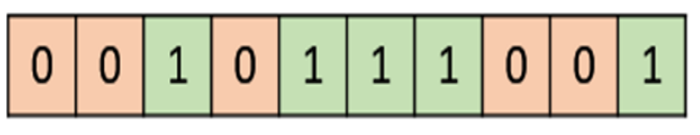
\includegraphics[scale=0.6]{binary_representation.PNG}
\caption{Mã hóa nhị phân}
\end{figure}  

\subsubsection{Mã hóa số thực}
Trong một số bài toán chúng ta muốn định nghĩa một cá thể bằng một vector với giá trị là liên tục thay vì các giá trị rời rạc, cách mã hóa số thực sẽ được sử dụng.
\begin{figure}[H]
\centering 
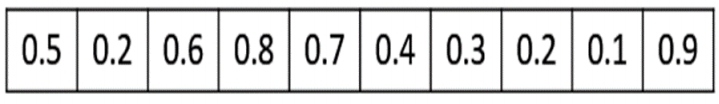
\includegraphics[scale=0.6]{real_representation.PNG}
\caption{Mã hóa số thực}
\end{figure}

\subsubsection{Mã hóa nguyên}
Với các bài toán lời giải là các giá trị rời rạc, ví dụ ta muốn mã hóa 4 hướng (Bắc, Nam, Đông, Tây), ta sẽ mã hóa chúng tương ứng với 4 số {1,2,3,4}. Trong trường hợp này, một cá thể sẽ được mã hóa bằng một vector các giá trị nguyên rời rạc (cụ thể là 4 số {1,2,3,4})
\begin{figure}[H]
\centering 
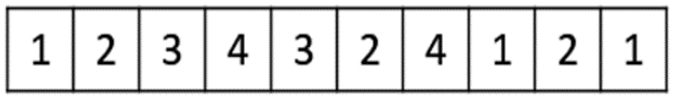
\includegraphics[scale=0.6]{integer_representation.PNG}
\caption{Mã hóa nguyên}
\end{figure}

\subsubsection{Mã hóa hoán vị}
Trong rất nhiều bài toán, lời giải sẽ được biểu diễn bởi một thứ tự các phần tử. Trong trường hợp đó, mã hóa hoán vị sẽ phù hợp cho mã hóa một cá thể.
\par Một ví điển hình trong trường hợp này là bài toán TSP (Travelling salesman problem): Một người du lịch xuất phát từ một thành phố và muốn thăm tất cả các thành phố, mỗi thành phố đúng 1 lần; cuối cùng quay lại thành phố xuất phát. Cần tìm một lịch trình sao cho tổng chi phí mà nguời du lịch phải bỏ ra là nhỏ nhất.
\par Nếu như đánh số các thành phố cần thăm từ 1->n (thành phố xuât phát là thành phố 0) thì lời giải của bài toán TSP là một hoán vị từ 1->n. Như vậy một cá thể sẽ được mã hóa là một vector x trong đó $x[0] = 0$; $x[n+1] = 0$ và $x[i] \in \{1,...,n\}$ 
\begin{figure}[H]
\centering
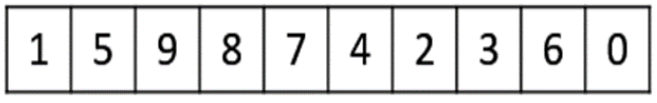
\includegraphics[scale=0.6]{permutation_representation.PNG}
\caption{Mã hóa hoán vị}
\end{figure}

\subsection{Một số toán tử lai ghép (Crossover)}
\subsubsection{One Point Crossover}
Mỗi cá thể trong quần thể có độ dài bằng nhau, ta sẽ chọn ngẫu nhiên một điểm và đổi chỗ phần đuôi của cha mẹ sinh ra 2 con mới. 
\begin{figure}[H]
\centering
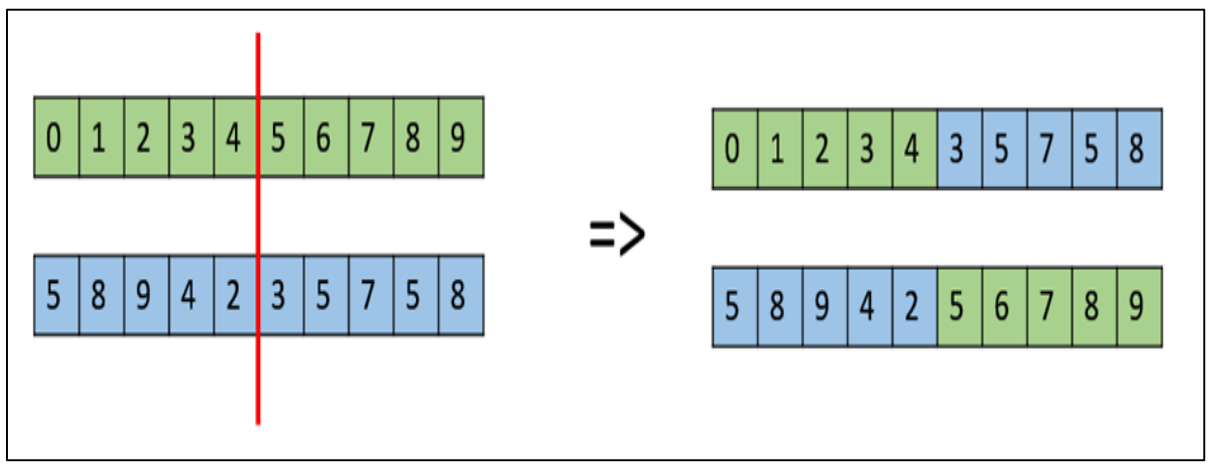
\includegraphics[scale=0.4]{one_point_crossover.png}
\caption{One Point Crossover}
\end{figure}

\subsubsection{Multi Point Crossover}
Lai ghép nhiều điểm cắt là trường hợp tổng quát của lai ghép một điểm cắt, ở đó các thành phần của cha và mẹ được đổi chỗ để tạo ra con mới.
\begin{figure}[H]
\centering
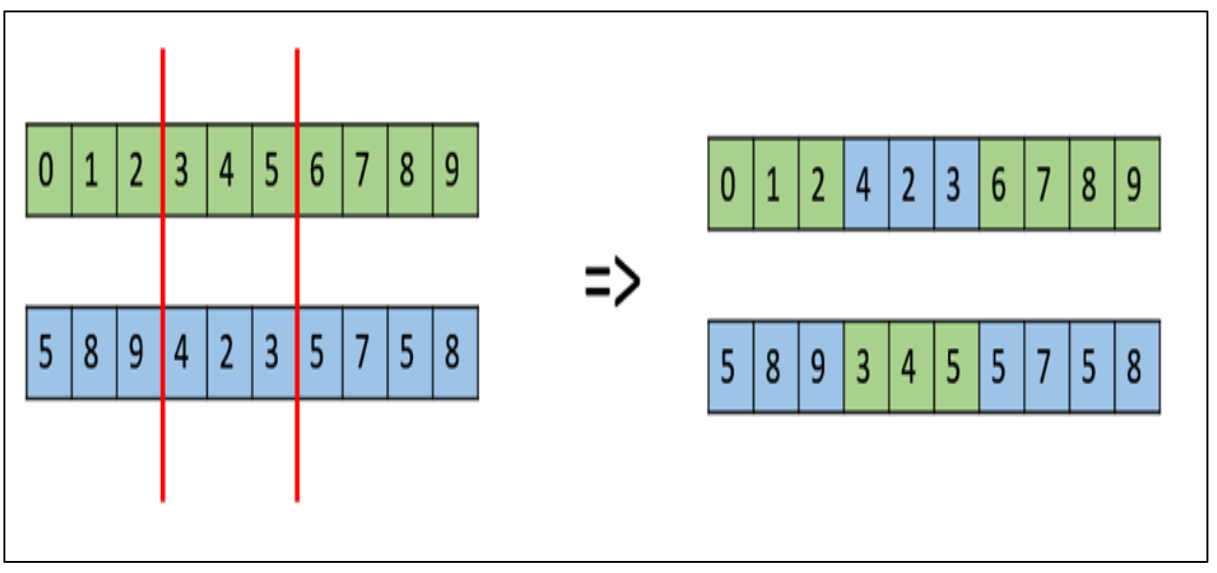
\includegraphics[scale=0.4]{multi_point_crossover.png}
\caption{Multi Point Crossover}
\end{figure}

\subsubsection{Whole Arithmetic Recombination}
Toán tử này thích hợp với cách mã hóa số thực. Cá thể con sinh ra sẽ được tính theo công thức:
\begin{itemize}
\item Child1 = a.parent1 + (1-a).parent2 
\item Child2 = a.parent2 + (1-a).parent1 
Trong đó a là một giá trị trong khoảng [0,1]
\end{itemize}
Nếu a = 0.5 thì 2 con sinh ra sẽ trùng nhau
\begin{figure}[H]
\centering 
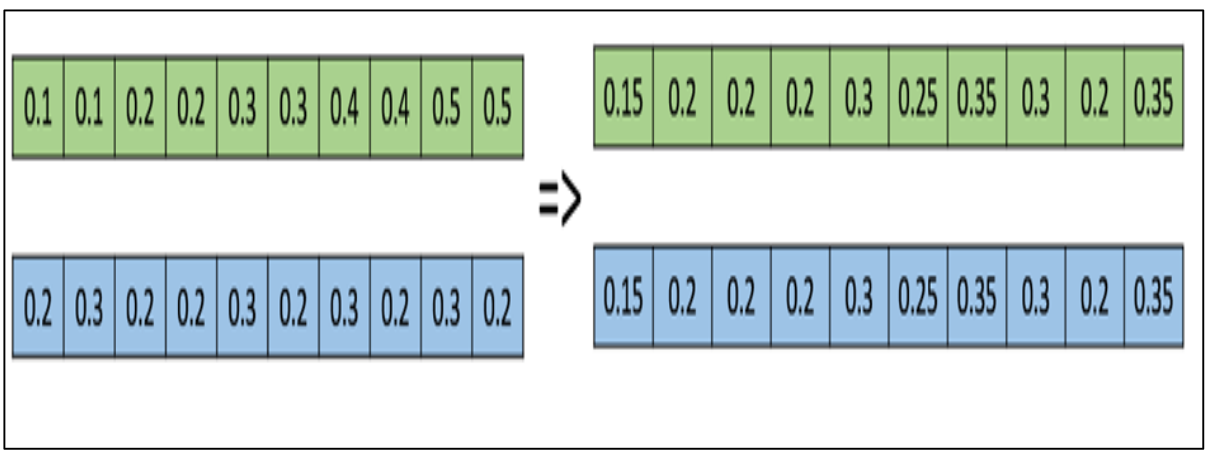
\includegraphics[scale=0.4]{whole_arithmetic_recombination.png}
\caption{Whole Arithmetic Recombination}
\end{figure}

\subsection{Một số toán tử đột biến (Mutation)}
\subsubsection{Bit Flip Mutation}
Trong toán tử đột biến đảo bit, ta chọn ngẫu nhiên 1 hay nhiều bit trong mã hóa của cá thể và đảo ngược bit được chọn.
\begin{figure}[H]
\centering
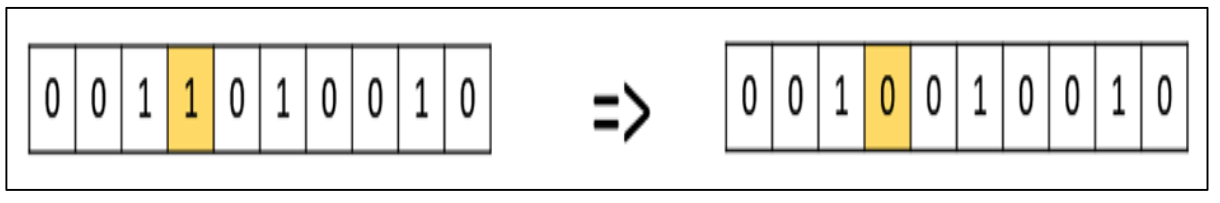
\includegraphics[scale=0.4]{bit_flip_mutation.png}
\caption{Bit Flip Mutation}
\end{figure}
 
\subsubsection{Random Resetting}
Lựa chọn ngẫu nhiên một phần tử trong một cá thể và chọn ngẫu nhiên một giá trị để thay thế
\begin{figure}[H]
\centering
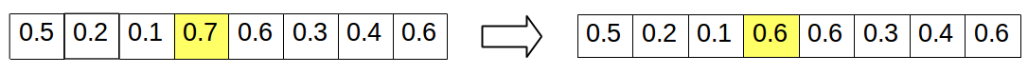
\includegraphics[scale=0.4]{random_resetting.png}
\caption{Random Resetting}
\end{figure}

\subsubsection{Swap Mutation}
Chọn ngẫu nhiên hai vị trí trong vector mã hóa của cá thể (nhiễm sắc thể) và đổi chỗ 2 vị trí cho nhau sẽ sinh ra con mới từ cá thể ban đầu
\begin{figure}[H]
\centering 
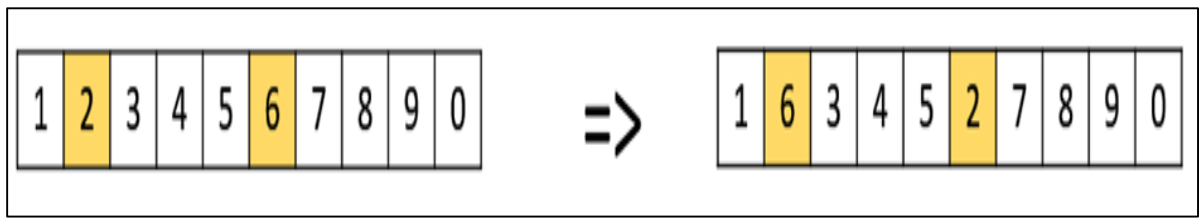
\includegraphics[scale=0.4]{swap_mutation.png}
\caption{Swap Mutation}
\end{figure}

\subsubsection{Scramble Mutation}
Scramble Mutation là một trong những cách đột biến thường dùng trong cách mã hóa hoán vị: Chọn ngẫu nhiên một tập nhỏ liên tiếp các gen (các phần tử liên tiếp trong một vector) và trộn gen đó với nhau để sinh ra con mới
\begin{figure}[H]
\centering 
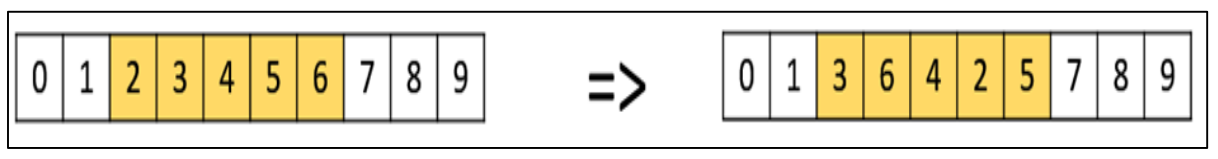
\includegraphics[scale=0.4]{scramble_mutation.png}
\caption{Scramble Mutation}
\end{figure}

\subsubsection{Inversion Mutation}
Chọn ngẫu nhiên một tập nhỏ các gen như trong scramble mutation, nhưng thay vì trộn các gen đó với nhau, ta đảo ngược lại thứ tự các gen đó.
\begin{figure}[H]
\centering 
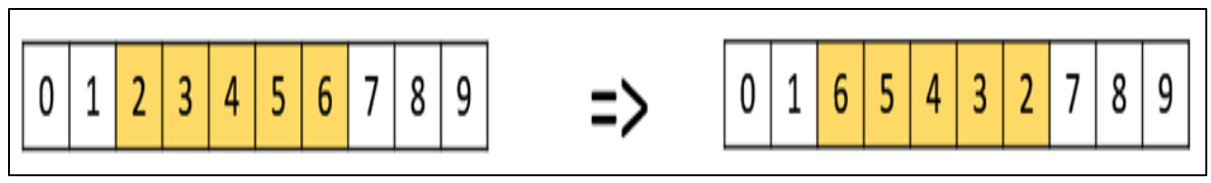
\includegraphics[scale=0.4]{inversion_mutation.png}
\caption{Inversion Mutation}
\end{figure}

\section{Tiến hóa đa nhiệm}\label{sec_mfo}
Giải thuật tiến hóa đã được áp dụng để giải nhiều bài toán tối ưu trong khoa học, trong kỹ thuật. Các bài tối ưu này thường được phân ra thành 2 nhóm: a) Tối ưu hóa đơn mục tiêu (single-objective optimization (SOO)), ở đó mỗi điểm trong không gian tìm kiếm được ánh xạ tới một giá trị vô hướng; b) Tối ưu hóa đa mục tiêu (multi-objective optimization (MOO)), ở đó mỗi điểm trong không gian tìm kiếm sẽ được ánh xạ tới một vector các hàm tối ưu. 
\par Trong phần này chúng em sẽ trình bày về một nhóm khác của bài toán tối ưu đó là bài toán tối ưu đa nhiệm (MutiFactorial Optimization (MFO)), tức tối ưu một bài toán với đầu vào của bài toán là nhiều bài toán tối ưu khác (khác với tối ưu hóa đa mục tiêu là một bài toán với nhiều hàm cần tối ưu). Để giải bài toán tối ưu đa nhiệm, trong phần này chúng em sẽ tìm hiểu về tiến hóa đa nhiệm.
\par Giả sử bài toán tối ưu đưa ra là cần tối ưu K bài toán (K task (giả sử cần tìm cực tiểu của các bài toán)). Task thứ $j^{th}$ ($T_j$) có không gian tìm kiếm lời giải $X_j$ và với hàm mục tiêu $f_j: X_j \rightarrow \mathbb{R}$. Thêm vào đó, lời giải của mỗi task cần thỏa mã một số ràng buộc (nếu có).
\par Như vậy quá trình tìm kiếm lời giải của bài toán là quá trình tìm kiếm bộ $\{x, x_1, x_2 ,..., x_K\}$ sao cho $\{x_1, x_2, ..., x_K\} = argmin \{f_1(x), f_2(x), ...., f_K(x)\}$ trong đó $x_j$ là một lời giải hợp lệ (thỏa mãn các ràng buộc) trong $X_j$, $x$ là lời giải (cách mã hóa) của bài toán đa nhiệm (cách mã hóa chung cho K bài toán cần tối ưu). Ở đó, mỗi hàm $f_j$ được xem như là một nhân tố ảnh hưởng tới sự tiến triển (cải thiện lời giải) của từng cá thể trong quần thể (nếu ta giải quyết bài toán theo giải thuật di truyền).
\par Để thiết kế giải thuật tiến hóa để giả bài toán MFO, ta cần định nghĩa hàm để so sánh độ tốt của các cá thể trong môi trường đa nhiệm (nhiều bài toán với mỗi bài toán lại có hàm mục tiêu khác nhau) (nếu như ở bài toán đơn mục tiêu, ta chỉ cần so sánh giá trị của hàm mục tiêu trên từng cá thể). Để định nghĩa được hàm so sánh giữa các cá thể, ta cần định nghĩa một vài thuộc tính của cá thể $p_i$ trong quần thể $P$ (trong đó $i \in \{1, 2, ..., |P|\}$). Chú ý rằng các cá thể sẽ được mã hóa trong một không gian đồng nhất (do cần tối ưu bài toán là hợp của $K$ bài toán con trong đó mỗi bài toán con lại có một không gian biểu diễn khác nhau $(X_1, X_2, ..., X_K$) và phải có cách giải mã một lời giải của bài toán thành lời giải của từng bài toán con (một cá thể $p_i$ thu được cần được giải mã bộ lời giải của $K$ bài toán con $\{{x_1}^i, {x_2}^i, ..., {x_K}^i\}$ trong đó ${x_1}^i \in X_1, {x_2}^i \in X_2, ..., {x_K}^i \in X_K$
\subsection{Một vài định nghĩa}
\begin{definition}[Factorial cost]
Với mỗi task $T_j$, factorial cost $\psi_j^i$ của $p_i$ được tính bởi công thức: $\psi_j^i = \lambda . \delta_j^i + f_j^i$ trong đó $\lambda$ là hằng số phạt, $f_j^i$ là giá trị hàm mục tiêu, $\delta_j^i$ là tổng các vi phạm ràng buộc của $p_i$ trên task $T_j$. Nếu $p_i$ là hợp lệ trên $T_j$ thì $\psi_j^i = f_j^i$
\end{definition}

\begin{definition}[Factorial rank]
Factorial rank $r_j^i$ của $p_i$ trên task $T_j$ là chỉ số của $p_i$ trong danh sách các cá thể trong quẩn thể $P$ sau khi được sắp xếp theo chiều tăng dần của 	factorial cost $\psi_j$
\end{definition}

\begin{definition}[Scalar fitness]
Danh sách của các factorial ranks $\{r_1^i, r_2^i, ..., r_K^i\}$ của cá thể $p_i$ sẽ được biến đổi thành một giá trị scalar fitness $\varphi_i$ phụ thuộc vào hạng cao nhất của $p_i$ trên $K$ task. $\varphi_i = \displaystyle\min_{j \in \{1,..,K\}} \{r_j^i\}$ 
\end{definition}

\begin{definition}[Skill factor]
skill factor $\tau_i$ của $p_i$ là một task trong số các task của bài toán MFO mà ở đó cá thể $p_i$ cho kết qủa tốt hơn cả. $\tau_i = argmin_j\{r_j^i\}$ trong đó $j \in \{1, 2, ..., K\}$
\end{definition}

\section{Giải thuật tiến hóa đa nhiệm (MFEA)}
\subsection{Sơ đồ chung của thuật toán}
\begin{figure}[H]
\centering 
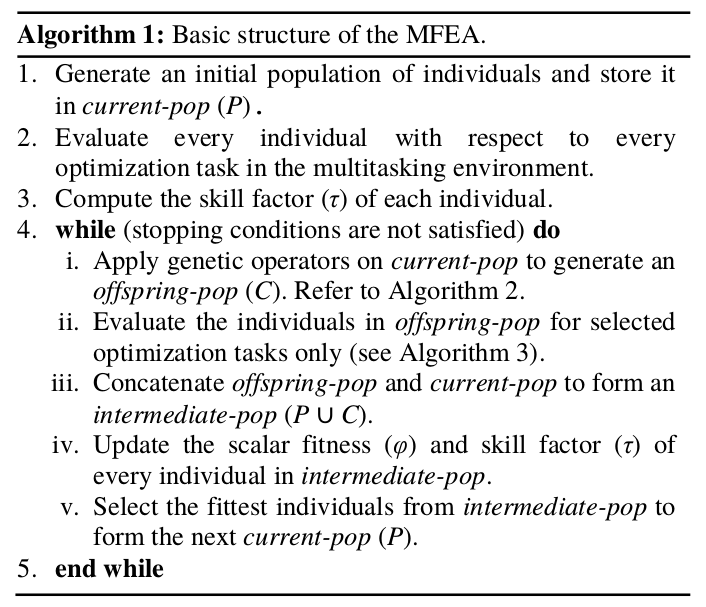
\includegraphics[scale=0.8]{al1.png}
\caption{Giải thuật MFEA - Sơ đồ chung}
\end{figure}
\begin{enumerate}
\item Cũng giống như giải thuật tiến hóa thông thường bước đầu tiên ta cần khởi tạo một quần thể gồm $n$ cá thể (các cá thể trong quần thể sẽ được mã hóa trong một không gian đồng nhất) và lưu trong biến \emph{current-pop (P)}.
\item Đánh giá từng cá thể trên từng task 
\item Tính skill factor ($\tau$) của mỗi cá thể
\item Cải thiện quần thể bằng cách áp dụng các toán tử đột biến, lai ghép để tạo ra cá thể mới, áp dụng các chiến thuật chọn lọc để tạo ra quần thể mới. 
\begin{enumerate}[i.]
\item Áp dụng các toán tử đột biến, lai ghép trên quần thể hiện tại  \emph{(current-pop)} để sinh ra các con \emph{(offspring-pop (C))}
\item Đánh giá từng cá thể trong các cá thể con mới được sinh ra \emph{(offspring-pop(C))} 
\item Hợp nhất các cá thể con mới sinh ra \emph{(offspring-pop(C))} vào quần thể hiện tại để tạo ra \emph{(intermediate-pop ($P \cup C$))} 
\item Cập nhật scalar fitness ($\varphi$) và skill factor ($\tau$) của mỗi cá thể trong \emph{(intermediate-pop ($P \cup C$))}
\item Chọn $n$ cá thể phù hợp nhất từ \emph{intermediate-pop} vào quần thể tiếp theo và gán lại vào biến \emph{current-pop}
\end{enumerate}
\end{enumerate} 

\subsection{Lai ghép, đột biến}
\begin{figure}[H]
\centering 
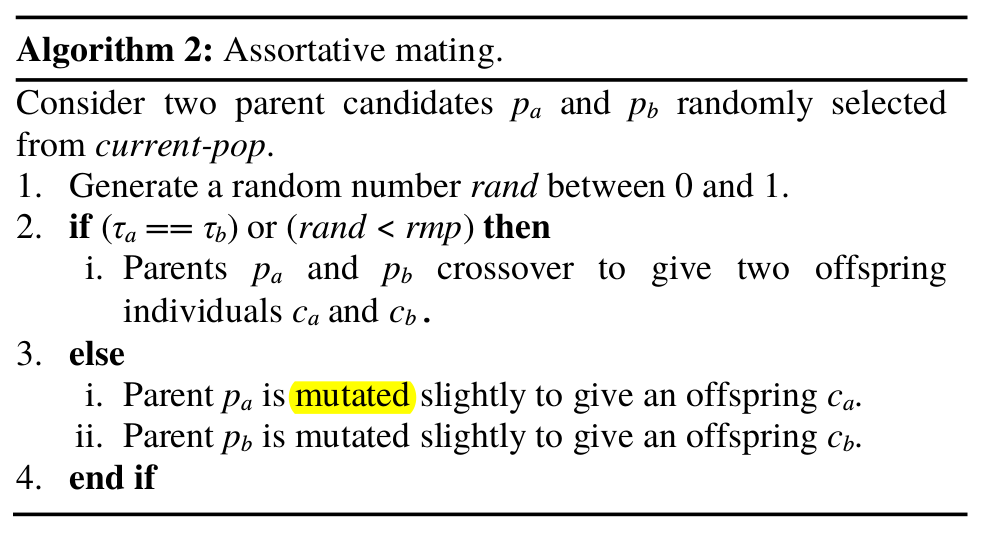
\includegraphics[scale=0.6]{al2.png}
\caption{Giả thật MFEA - Lai ghép, đột biến}
\end{figure}  
Lựa chọn ngẫu nhiên 2 cá thể cha mẹ $p_a$ và $p_b$ trong quần thể hiện tại (\emph{current-pop})
\begin{enumerate}
\item Sinh ngẫu nhiên một số trong khoảng [0,1] 
\item Nếu skill factor của 2 cá thể cha mẹ bằng nhau hoặc số sinh ngẫu nhiên trong khoảng [0,1] nhỏ hơn ngưỡng định sẵn nào đó thì $p_a$ và $p_b$ sẽ được lai ghép tạo ra 2 con mới $c_a$ và $c_b$
\item Nếu không 
\begin{enumerate}[i.]
\item $p_a$ sẽ được đột biến sinh ra con $c_a$
\item $p_b$ sẽ được đột biến sinh ra con $c_b$
\end{enumerate}
\end{enumerate}

\subsection{Đánh giá cá thể}
\begin{figure}[H]
\centering 
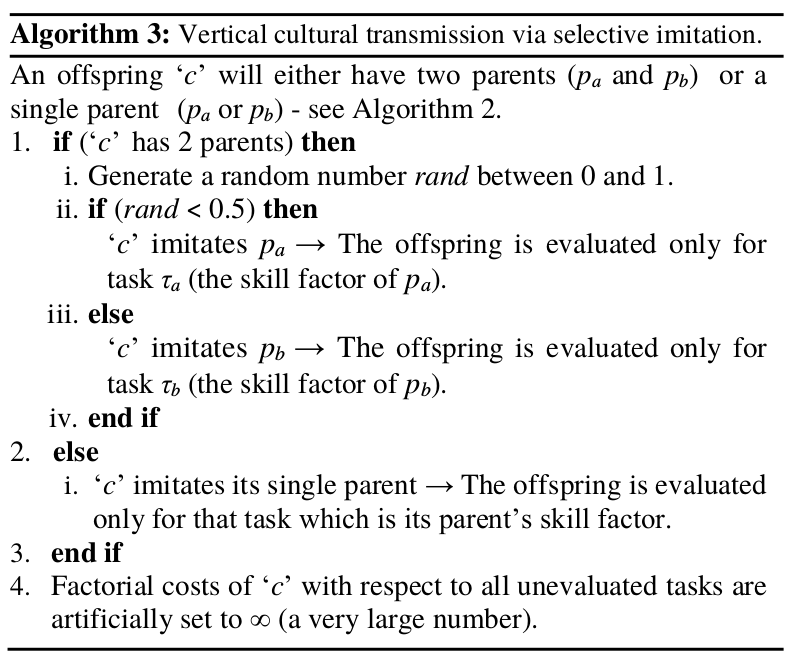
\includegraphics[scale=0.7]{al3.png}
\caption{Giả thật MFEA - Đánh giá cá thể }
\end{figure} 
Một con $c$ mới được sinh ra sẽ là con của một cha một mẹ $p_a$ và $p_b$ khi đem lai ghép hoặc là con của hoặc cha hoặc mẹ $p_a$ hoặc $p_b$ khi đem đột biến.
\begin{enumerate}
\item Nếu $c$ có một cha một mẹ 
\begin{enumerate}[i.]
\item Sinh một số ngẫu nhiên trong khoảng [0,1]
\item Nếu số sinh ngẫu nhiên nhỏ hơn 0.5 thì $c$ sẽ được đánh giá dựa trên task $\tau_a$ (skill factor của $p_a$)
\item Nếu không skill factor của $c$ sẽ được đánh giá dựa trên task $\tau_b$ (skill factor của $p_b$)
\end{enumerate}
\item Nếu $c$ chỉ có hoặc cha hoặc mẹ thì $c$ sẽ được đánh giá dựa trên task bằng giá trị của skill factor của cha hoặc mẹ sinh ra $c$
\end{enumerate}

\chapter{Ứng dụng}
\section{Bài toán ứng dụng}
\subsection{Bài toán Người Du Lịch(TSP)}
Đầu vào của bài toán là tập các thành phố và khoảng cách giữa mỗi cặp thành phố, đầu ra của bài toán là một hành trình thỏa mãn đi qua tất cả các thành phố và mỗi thành phố được thăm đúng một lần và có độ dài của hành trình là nhỏ nhất.\\

\begin{figure}[H]
\center
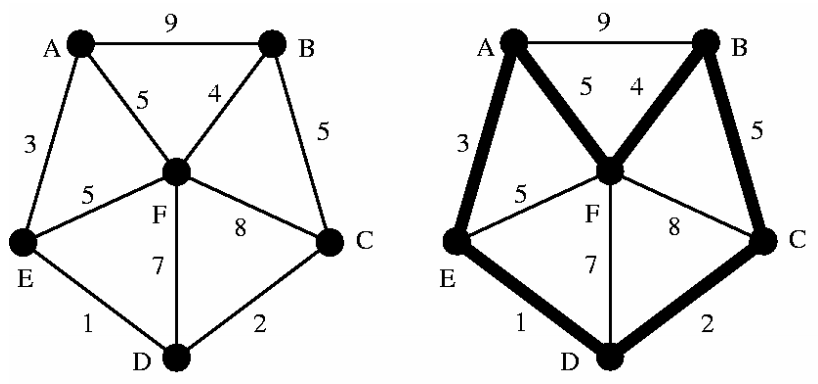
\includegraphics[scale=0.5]{TSP_example.PNG}
\caption{Ví dụ bài toán TSP}
\end{figure}

TSP là bài toán NP-hard trong lĩnh vực tối ưu hóa tổ hợp.
\subsection{Bài toán cái túi}
Bài toán cái túi: Cần chất các đồ vật vào một cái túi có trọng lượng ($b$), mỗi đồ vật có hai thông số về trọng lượng ($b_i$) và giá trị sử dụng ($w_i$). Đầu ra của bài toán là một tập con các đồ vật sao cho tổng trọng lượng của các đồ vật trong tập nhỏ hơn hoặc bằng trọng lượng của túi ($b$) và tổng giá trị của các đồ vật trong tập có giá trị lớn nhất.
\begin{figure}[H]
\center
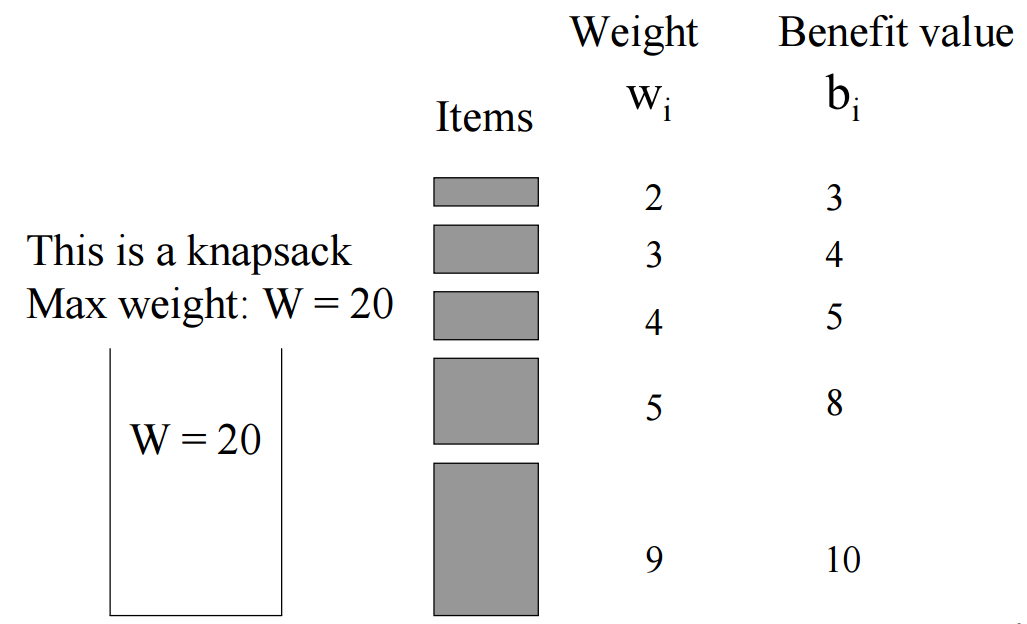
\includegraphics[scale=0.5]{KP_example.PNG}
\caption{Ví dụ bài toán cái túi}
\end{figure}

\subsection{Cách mã hóa cá thể}
Như đã đề cập ở phần \ref{sec_mfo}, làm thế nào để mã hóa một cá thể trong một không gian đồng nhất trong khi đầu vào của bài toán là $K$ bài toán con ở đó mỗi bài toán con lại có một không gian biểu diễn lời giải khác nhau.
\par Giả sử lời giải của task $T_j$ khi biểu diễn trong bài toán tối ưu đơn nhiệm (đơn mục tiêu và đa mục tiêu) được mã hóa bởi một vector có số chiều $D_j$. Ta sẽ mã hóa mỗi cá thể trong bài toán MFO bằng một vector có số chiều bằng $D = max\{D_j\}$. Sau đó ta có thể áp dụng các cách mã hóa đã trình bày ở mục \ref{sub_encode}  để mã hóa và tương ứng với mỗi cách mã hóa ta sẽ phải tìm cách giải mã sao cho từ một cá thể trong không gian đồng nhất với mỗi bài toán con có cách giải mã ra lời giải của từng bài toán đó. Trong bài báo cáo này, chúng em lựa chọn cách mã hóa số thực để biểu diễn cá thể
\subsubsection{Mã hóa}
Mỗi cá thể sẽ được mã hóa bởi một vector có số chiều $D = max\{D_j\}$ và có giá trị là các số thực trong khoảng $[0,1]$. Xét ví dụ: mã hóa bài toán gồm 2 task: TSP (6 thành phố) và bài toán cái túi nhị phân (12 đồ vật).
\par Một cá thể của bài toán TSP (6 thành phố) trong bài toán tối ưu đơn nhiệm sẽ được mã hóa bằng một vector có số chiều bằng 6 và giá trị của vector thông thường sẽ là hoán vị của các số từ 1 đến 6 (tương ứng với thứ tự thăm của các thành phố). Còn một cá thể của bài toán cái túi nhị phân (12 đồ vật) trong bài toán tối ưu đơn nhiệm sẽ được mã hóa bằng một vector $x$ có số chiều bằng 12 và giá trị của vector là các số nhị phân 0 hoặc 1 ($x_i=1$ tức đồ vật $i$ sẽ được xếp vào túi). Như vậy khi một cá thể trong bài toán MFO sẽ được mã hóa bằng một vector có số chiều là $D = max\{D_j\} = 12$ do chúng em chọn cách mã hóa số thực nên giá trị của vector là các số thực trong khoảng [0,1]. Ví dụ một cá thể \cite{MFO-slide}
\begin{longtable}{|c|c|c|c|c|c|c|c|c|c|c|c|}
\hline
0.8 & 0.9 & 0.1 & 0.9 & 0.6 & 0.0 & 0.2 & 0.5 & 0.9 & 0.4 & 0.1 & 0.9\\
\hline
\end{longtable}

\subsubsection{Giải mã}
Từ một cá thể trong không gian đồng nhất với mỗi bài toán con cần chọn cách giải mã ra lời giải của từng bài toán đó bằng cách với mỗi bài toán con có lời giải là vector $k$ chiều thì sẽ lấy k giá trị đầu tiên trong vector biểu diễn cá thể trong bài toán MFO và tìm cách giải mã thành lời giải hợp lệ của bài toán con đó. Với ví dụ trên: 
\begin{itemize}
\item Với bài toán TSP cần giải mã ra một vector độ dài 6 gồm các giá trị là một hoán vị của các số từ 1 đến 6. Ta sẽ chọn 6 số đầu tiên trong cá thể của bài toán MFO là \{0.8,0.9,0.1,0.9,0.6,0.0\} (dãy 1) và cần tìm cách giải mã dãy này về một dãy hoán vị của các số từ 1 đến 6 bằng cách: Sắp xếp dãy \{0.8,0.9,0.1,0.9,0.6,0.0\} theo thứ tự tăng dần (\{0.0, 0.1, 0.6, 0.8, 0.9, 0.9\} (dãy 2)) rồi duyệt qua các phần tử của dãy 2. Với mỗi phần tử, vị trí của nó trong dãy 1 sẽ là giá trị của vector lời giải của bài toán TSP. Ví dụ phần tử 0.0 trong dãy 2 đứng thứ 6 trong dãy 1 nên vị trí thứ nhất trong vector lời giải của bài toán TSP là 6; cứ làm nhưu vậy ta sẽ được một vector là lời giải của bài toán TSP sau khi giải mã vector biểu diễn cá thể của bài toán MFO trong ví dụ trên là :
\begin{longtable}{|c|c|c|c|c|c|}
\hline
6& 3& 5& 1& 2& 4\\
\hline
\end{longtable}

\item Với bài toán cái túi cần giải mã ra một vector có độ dài 12 gồm các giá trị là 0 hoặc 1. Vì vậy chỉ cần lấy phần nguyên già của từng phần tử trong vector biểu diễn cá thể của bài toán MFO sẽ được một vector lời giải của bài toán cái túi như sau:
\begin{longtable}{|c|c|c|c|c|c|c|c|c|c|c|c|}
\hline
1& 1& 0& 1& 1& 0&0&1&1&0&0&1\\
\hline
\end{longtable}
Tuy nhiên ta cần kiểm tra vector có thỏa mãn điều kiện của bài toán không (tổng trọng lượng của các đồ vật phải nhỏ hơn trọng lượng của cái túi). Nếu vector giải mã không thỏa mãn điều kiện của bài toán cái túi (trọng lượng của các đồ vật lớn hơn trọng lượng của cái túi) ta cần chọn một số đồ vật để bỏ bớt ra khỏi túi (trong cài đặt chúng em chọn các đồ vật có trọng số ($w_i/b_i$ là nhỏ nhất)) bằng cách đặt giá trị tương ứng với chỉ số của đồ vật đó trong vector biểu diễn cá thể của bài toán MFO là một giá trị nhỏ hơn 0.5 (dẫn đến khi giải mã giá trị tại vị trí đó bằng 0 tức là không chất đồ vật đó vào túi).  
\end{itemize}

\subsection{Cải tiến áp dụng tích chập để lưu giữ đặc trưng}
Với cách giải mã ở trên, ta có thể nhận thấy bài toán có lời giải biểu diễn bởi một vector có số chiều ngắn hơn sẽ "thiệt thòi" hơn do chỉ được sử dụng một phần của vector biểu diễn cá thể của bài toán MFO. Vì vậy chúng em đề xuất sử dụng "tích chập" để có thể trích toàn bộ đặc trưng (sử dụng toàn bộ giá trị) của vector biểu diễn cá thể của bài toán MFO. 
\par Cụ thể thay vì với mỗi bài toán có lời giải biểu diễn bởi một vector $k$ chiều chỉ lấy $k$ giá trị đầu tiên của vector biểu diễn cá thể của bài toán MFO, thì chúng em thêm một vector (gọi là cửa sổ trượt) trượt qua toàn bộ vector biểu diễn cá thể của bài toán MFO để có thể thu được vector lời giải của bài toán con. 
\par Giả sử vector biểu diễn cá thể của bài toán MFO có dạng:
\begin{longtable}{|c|c|c|c|c|c|}
\hline
$x_1$ & $x_2$ & $x_3$ & ... & $x_{n-1}$ & $x_n$ \\
\hline
\end{longtable}

\par Vector cửa sổ trượt có dạng 
\begin{longtable}{|c|c|c|}
\hline
$w_1$ & $w_2$ & $w_3$\\
\hline
\end{longtable}
\par Ta sẽ thu được vector lời giải của bài toán con có dạng (giả sử bước nhảy của cửa sổ là 2)
\begin{longtable}{|c|c|c|c|c|}
\hline
$x_1*w_1+x_2*w_2+x_3*w_3$ & $x_3*w_1+x_4*w_2+x_5*w_3$ &... & $x_i*w_1+x_{i+1}*w_2+x_{i+2}*w_3$ & ...\\
\hline
\end{longtable}

\par Có thể nhận thấy có trường hợp khi đến cuối vector biểu diễn cá thể của bài toán MFO, cửa sổ có thể bị chờm ra ngoài, trong trong trường hợp đó, ta sẽ thêm vào vector biểu diễn cá thể của bài toán MFO những số thực ngẫu nhiên trong khoảng [0,1]. Và để đảm bảo vector lời giải của bài toán con có đủ $k$ chiều ta sẽ chọn số lượng số thực được thêm vào cuối vector biểu diễn cá thể của bài toán MFO và bước nhảy của cửa sổ sao cho thỏa mãn công thức:  
$$D' = (D-F+P)/S + 1$$
\begin{itemize}
\item $D'$ : số chiều của vector lời giải của bài toán con
\item $D$ : số chiều của cá thể biểu biễn bài toán MFO 
\item $F$ : số chiều của vector cửa sổ 
\item $P$ : số lượng số thực được thêm vào cuối vector biểu diễn cá thể bài toán MFO
\item $S$ : bước nhảy của cửa sổ   
\end{itemize}
\par Ta cần chọn S và P:
\begin{itemize}
\item Nếu $(D'-1)$ chia hết cho $(D-F)$ thì $S = \frac{D'-1}{D-F}$ và $P=0$
\item Nếu $(D'-1)$ không chia hết cho $(D-F)$ thì $S =  \lfloor \frac{D'-1}{D-F} \rfloor$  và $P = (D'-1)*S - D + F$ 
\end{itemize}

\section{Cài đặt} 
Trong phần này chúng em sẽ trình bày một số hàm quan trọng trong cài đặt của thuật toán MFEA 
\subsection{Hàm kiểm tra tính hợp lệ của cá thể}
Với bài toán cái túi trường hợp sau khi giải mã được một vector không thỏa mãn ràng buộc về khối lượng . 
\begin{lstlisting}
public void makeIndividualVail(ArrayList<Double> ind){
	int i=0;
	int xd=0;	
	while(true){
		Task t= tasks.get(i);
		if(!t.checkIndivialVail(ind)){// kiem tra xem ca the co		
									  // hop le khong
			xd=0;
			t.makeIndivialVail(ind); //lam cho ca the hop le
		} else {
			xd++;
		}
		if(xd>=tasks.size()){ // lap lai cho den khi tat ca task
			break;            // deu hop le
		}
		i=(i+1)%tasks.size();
	}
}
	
\end{lstlisting}
Loại bỏ từ kiểu gen lần lượt các phần tử có tỉ số giữa giá trị trên khối lượng lớn dần đén khi cá thể hợp lệ.
\begin{lstlisting}
public ArrayList<Double> makeIndivialVail(ArrayList<Double> x){
		double wx=getWeight(decode(x));
		int i=0;
		Random r= new Random();
		while(wx>b){
			if(Math.round( x.get(vtcw[i]))==1){
				wx=wx-w[vtcw[i]];
			}
			x.set(vtcw[i], r.nextDouble()*5/10);
			i++;
		}
		return x;
}
\end{lstlisting}
\begin{itemize}
\item 
\end{itemize}
\section{Kết quả thực tế}

\textbf{Kiểu lai ghép} : Lai ghép một điểm cắt


\begin{longtable}{|l |c |c |c |c|}
\hline
\multirow{2}{*}{Test} 
& \multicolumn{2}{c|}{Not Covl} &\multicolumn{2}{|c|}{Covl} \\
\cline{2-5}
&TSP & Knapsack & TSP & KnapSack \\
\hline
kp200-tsp20  & 551.9&29541 &545 &28081 
\\ \hline
kp200-tsp52&22412 &28939&19728 &27909 \\ \hline
kp1000-tsp20 &560.6&69707&552&68789 \\ \hline
kp1000-tsp52 &22832&70815&20176&69856 \\ \hline
kp20000-tsp20 &562&388917&517 &391661 \\ \hline
kp20000-tsp52 &21327&390872&22234& 388777\\ \hline
\end{longtable}

\textbf{Kiểu lai ghép} : Lai ghép nhiều điểm cắt

\begin{longtable}{|l |c |c |c |c|}
\hline
\multirow{2}{*}{Test} 
& \multicolumn{2}{c|}{Not Covl} &\multicolumn{2}{|c|}{Covl} \\
\cline{2-5}
&TSP & Knapsack & TSP & KnapSack \\
\hline
kp200-tsp20  & 584&29041 &537 &27703 
\\ \hline
kp200-tsp52&22158 &28939&28660 &28378 \\ \hline
kp1000-tsp20 &586&70319&516&70563 \\ \hline
kp1000-tsp52 &23400&69709&19793&69157 \\ \hline
kp20000-tsp20 &545&387700&545 &386705 \\ \hline
kp20000-tsp52 &21975&386778&21511& 390374\\ \hline
\end{longtable}
\textbf{Kiểu đột biến} : Đổi biến đổi chỗ.

\begin{longtable}{|l |c |c |c |c|}
\hline
\multirow{2}{*}{Test} 
& \multicolumn{2}{c|}{Not Covl} &\multicolumn{2}{|c|}{Covl} \\
\cline{2-5}
&TSP & Knapsack & TSP & KnapSack \\
\hline
kp200-tsp20  & 561&27588 &533 &28751 
\\ \hline
kp200-tsp52&22651 &28411&20805 &29609 \\ \hline
kp1000-tsp20 &576&69879&516&69170 \\ \hline
kp1000-tsp52 &22971&69648&20761&70671 \\ \hline
kp20000-tsp20 &572&385427&527 &386705 \\ \hline

kp20000-tsp52 &22426 & 389005 & 21437 & 386637\\
\hline
\end{longtable}
\begin{thebibliography}{9}
\bibitem{TSP} \url{http://ccf.ee.ntu.edu.tw/~cchen/course/simulation/CAD/unit1A.pdf}

\bibitem{GA} Tutorialspoint, \textit{Genetic Algorithms Tutorial}

\bibitem{MFO} Abhishek Gupta, Yew-Soon Ong, and Liang Feng; \textit{Multifactorial Evolution: Towards Evolutionary Multitasking}

\bibitem{MFO-slide} Yew-Soon Ong, \textit{Multifactorial Optimization: Towards Evolutionary Multitasking (Presentation)} 

\end{thebibliography}


\end{document}
